\section{Wikipedia assignment: EE 102 in the wild}
This year in EE 102, we are exploring a new way to learn concepts related to signal processing by connecting it to the real world. We will do this by editing Wikipedia articles related to EE 102. This Wikipedia assignment will help you connect EE 102 with applications, people, instruments, and
ideas beyond our lectures. You have been assigned a team at random on CatCourses. Each team will learn about a signal processing
topic, research published sources, and contribute a clear, well-supported
writeup (with sources) to its Wikipedia article. You are writing for readers outside this
class and helping them understand something you have learned.

\textbf{Grading}: The Wikipedia assignment is part of Midterm \#3. The Wikipedia assignment contributes
\textbf{20 points}, and the written exam contributes \textbf{80 points}.

\subsection{First step: Register on the course dashboard}
Last week's announcement introduced the assignment. If you have not
registered yet, please get started now:
\begin{enumerate}
    \item Find your team in
    \href{https://catcourses.ucmerced.edu/courses/39201/groups\#tab-9972}{the CatCourses group list}.
    \item Create or sign in to your own Wikipedia account and
    \href{https://dashboard.wikiedu.org/courses/UC_Merced/Signal_Processing_and_Linear_Systems_(Fall_2026)?enroll=kzbshpao}{enroll in our Wiki Education course dashboard}.
    Each team member should enroll.
    \item Start the
    \href{https://dashboard.wikiedu.org/training/students/wikipedia-essentials}{Wikipedia policies training module}
    linked in the announcement. Then follow the assigned training and
    activities on our dashboard.
\end{enumerate}

The activities of this week on the Wiki Education dashboard that are due this week are shown in the image below:
\begin{figure}[t]
    \centering
    
\includegraphics[width=0.5\textwidth]{wikipedia_assignment_week10_tasks.png}
    \caption{The Wiki Education dashboard shows the activities assigned to our course.}
    \label{fig:dashboard}
\end{figure}



\subsection{Possible topics for EE 102}
You can explore topics we have not yet studied in detail. Look for a clear
connection to signals, systems, frequency content, or the history of these
ideas. Some possible directions could be:
\begin{itemize}
    \item \textbf{Audio and music:} pitch, timbre, noise reduction, or the
    \href{https://en.wikipedia.org/wiki/Phase_vocoder}{phase vocoder}.
    Research how time- and frequency-domain descriptions support a specific
    audio technique or application.
    \item \textbf{Scientific instruments:} lock-in amplifier,
    oscilloscopes, or spectrum analyzers. Explore how an instrument extracts
    useful information from a measured signal.
    \item \textbf{Signals in other fields:} EEG/ECG recordings, seismic
    signals, or sonar. A focused application can connect our mathematical
    tools to measurements and questions in another discipline.
    \item \textbf{History and people:} the development of harmonic analysis,
    early sound-analysis instruments, or a documented contribution to
    signal-processing history. Research the context and evidence behind
    the development, as well as the technical idea.
\end{itemize}

\section{Midterm course feedback}
Please fill out the survey called \textbf{Midterm course feedback} when it
is launched on CatCourses. Use it to share what is helping you learn and
what could improve the second half of the course.


\section{Goals}
The overall goal in EE 102 is to break down signals into its constituent fundamental components that can be easily analyzed. So far, we have achieved this in two ways: we have broken down any arbitrary signal into impulse signals, and we have broken down periodic signals into sinusoids. What's left? Signals that are not periodic. So, our goal is \dots 

By the end of this lecture, you should be able to break down aperiodic signals into their constituent frequency components using Fourier Transform.
% ---------- Pop-Quiz 1 ----------
\section{Practice problems: Decomposition of signals}
In this section, we review how to decompose signals into simpler components. We have already seen two ways to do this: using impulses and using sinusoids. We will work through one example of each. 
\subsection{Breaking down signals using impulses}
Choose a signal $x(t)$ --- scribble something! Break it down so that it can be constructed using only impulses $\delta(t)$ with appropriate scales and shifts.

\medskip
\textbf{(a) Show it visually: } On the left, sketch $x(t)$. On the right, place weighted impulses at sample locations corresponding to the value of $x(t)$ at those locations. Note that integer times are shown here, but you may choose any sampling interval (can be floating point because this is a continuous-time signal).

\begin{center}
\begin{minipage}{0.47\linewidth}
\begin{tikzpicture}[x=0.7cm,y=0.9cm]
  \draw[->] (-4.6,0) -- (4.6,0) node[below] {$t$};
  \draw[->] (0,-2.2) -- (0,2.6) node[left] {$x(t)$};
  \foreach \xx in {-4,-3,-2,-1,1,2,3,4}{\fill[black!25] (\xx,0) circle(0.03);}
  \foreach \yy in {-2,-1,1,2}{\fill[black!25] (0,\yy) circle(0.03);}
  \node[align=center] at (0,3.2) {\small Sketch $x(t)$ here};
\end{tikzpicture}
\end{minipage}\hfill
\begin{minipage}{0.47\linewidth}
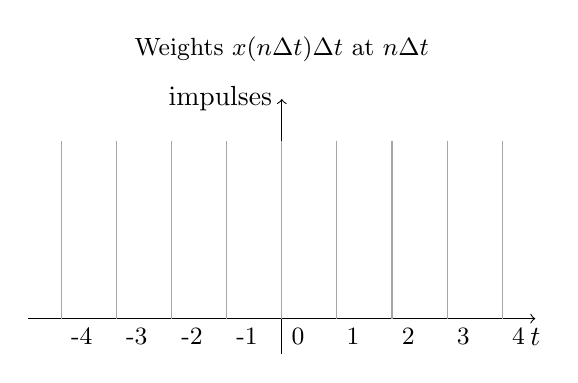
\begin{tikzpicture}[x=0.7cm,y=0.9cm]
  \draw[->] (-4.6,0) -- (4.6,0) node[below] {$t$};
  \draw[->] (0,-0.5) -- (0,3.1) node[left] {impulses};
  \foreach \n in {-4,-3,-2,-1,0,1,2,3,4}{
     \draw[black!35] (\n,0) -- ++(0,2.5);
     \node[below right] at (\n,0) {\small \n};
  }
  \node[align=center] at (0,3.8) {\small Weights $x(n\Delta t)\Delta t$ at $n\Delta t$};
\end{tikzpicture}
\end{minipage}
\end{center}

\medskip
\textbf{(b) Do it mathematically:} Use the sifting property to write a formula for $x(t)$ using $\delta(\cdot)$.

\fbox{\begin{minipage}[t][3.0cm][t]{0.98\linewidth}
\vspace{0.2cm}
\textit{Write your mathematical expression here:}
\end{minipage}}

\textbf{Possible solution}
We sketch $x(t)$ as a continuous curve on the left, and place impulses at various locations, which is shown on the right. 
\begin{center}
\begin{minipage}{0.47\linewidth}
\begin{tikzpicture}[x=0.7cm,y=0.9cm]
  \draw[->] (-4.6,0) -- (4.6,0) node[below] {$t$};
  \draw[->] (0,-2.2) -- (0,2.6) node[left] {$x(t)$};
  \draw[very thick] (-4,0.2) .. controls (-2,1.6) and (-1.2,1.8) .. (0,0.3)
                     .. controls (0.7,-0.2) and (2,0.8) .. (3.3,1.6)
                     .. controls (3.7,1.9) and (4.2,1.2) .. (4.3,0.1);
\end{tikzpicture}
\end{minipage}\hfill
\begin{minipage}{0.47\linewidth}
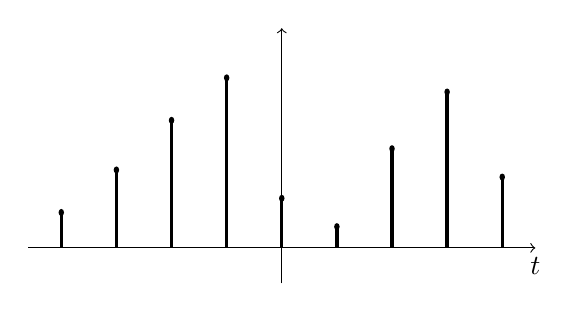
\begin{tikzpicture}[x=0.7cm,y=0.9cm]
  \draw[->] (-4.6,0) -- (4.6,0) node[below] {$t$};
  \draw[->] (0,-0.5) -- (0,3.1);
  \foreach \n/\h in {-4/0.5,-3/1.1,-2/1.8,-1/2.4,0/0.7,1/0.3,2/1.4,3/2.2,4/1.0}{
     \draw[very thick] (\n,0) -- ++(0,\h);
     \fill (\n,\h) circle(0.05);
  }
\end{tikzpicture}
\end{minipage}
\end{center}

Mathematically, we have the sifting property of the impulse:
\[\,x(t)=\int_{-\infty}^{\infty} x(\tau)\,\delta(t-\tau)\,d\tau\,
\] 

\subsection{Breaking down periodic signals using sinusoids}
Draw an impulse train with period $T_0$. Then, sketch (approximately) how a finite sum of sinusoids could approximate this train over time (recall the virutal manipulator we explored for Fourier Series in week 7 or your work on Desmos Graphing Calculator). Finally, write the corresponding Fourier-series form and coefficients.

\fbox{\begin{minipage}[t][3.0cm][t]{0.98\linewidth}
\vspace{0.2cm}
\textit{Write $x(t)=\sum_{k=-\infty}^{\infty} a_k e^{jk\omega_0 t}$ and specify $a_k$. Optionally write the finite $N$-term partial sum you would draw.}
\end{minipage}}


Finally, consider a $50\%$ duty cycle symmetric square wave of amplitude $A$ and period $T_0=\dfrac{2\pi}{\omega_0}$. Sketch one period on an axes, draw the first few nonzero harmonic magnitudes, and write the Fourier series formula you would use to represent this signal.
% \textbf{(b)} On the right, draw the first few harmonic magnitudes (only nonzero ones).

\fbox{\begin{minipage}[t][3.2cm][t]{0.98\linewidth}
\vspace{0.2cm}
\textit{Write the FS synthesis and coefficients. State your levels ($0,A$ or $-A,A$) and time origin.}
\end{minipage}}

\paragraph{Why/how is that useful?}

After you have worked through the above examples, you are all set up to compute the output of any LTI system. To achieve that you would need the following additional information (one or the other): 
\begin{itemize}
    \item How does the system respond to an impulse input? (i.e., the impulse response of the system, $h(t)$)
    \item How does the system respond to sinusoidal inputs? (i.e., the frequency response of the system, $H(j\omega)$)
\end{itemize}
Then, you can compute the output of the system for any arbitrary input signal $x(t)$ using either convolution or the Fourier synthesis equation (and LTI system properties!).

\section{Fourier Transform: Decomposition of aperiodic signals}
The question we set for ourselves at the beginning was: how do we break down aperiodic signals into their constituent frequency components?

The \ul{\textbf{key idea}} is to break down an aperiodic signal, first write its periodic extension by repeating the signal over and over. Then, we will argue that as the time period increases, the signal grows more and more further apart, until as $T\to\infty$, the signal becomes aperiodic. In other words, we can think of an aperiodic signal as the limit of periodic signals with increasingly large periods.

\subsection{Example: An aperiodic rectangular pulse} 
To build this idea, let us consider an example of a rectangular pulse. Consider repetitions of a single rectangular pulse and then let their period $T \to \infty$. Then, on any fixed finite time interval, sufficiently distant repetitions disappear from view, giving us back our aperiodic signal.

Let us define the rectangular pulse mathematically. We have a periodic rectangular pulse train of height $A$, period $T$, and fixed pulse width $2T_1<T$. For the period between $-T/2$ and $T/2$, the signal is defined as:
\[
x(t) = \begin{cases}
A, & -T_1 \le t \le T_1,\\
0, & \text{otherwise.}
\end{cases}
\]
We can find the Fourier series coefficients for this signal using the Fourier series analysis equation:
\[
a_k = \frac{1}{T} \int_{-T/2}^{T/2} x(t) e^{-jk\omega_0 t} dt,
\]
where $\omega_0 = \dfrac{2\pi}{T}$. Note that the limits of integration should be (ideally, according to the formula for $a_k$) over one period of the signal. However, since $x(t)$ is zero outside the interval $[-T_1, T_1]$, we can simplify the limits of integration to:
\[
a_k = \frac{1}{T} \int_{-T_1}^{T_1} A e^{-jk\omega_0 t} dt.
\]
For $k\ne0$, evaluating this integral gives:
\begin{align*}
    a_k &= \frac{A}{T} \int_{-T_1}^{T_1} e^{-jk\omega_0 t} dt \\
    &= \frac{A}{T} \left[ \frac{e^{-jk\omega_0 t}}{-jk\omega_0} \right]_{-T_1}^{T_1} \\
    &= \frac{A}{T} \left( \frac{e^{-jk\omega_0 T_1} - e^{jk\omega_0 T_1}}{-jk\omega_0} \right) \\
    &= \frac{A}{T} \left( \frac{-2j \sin(k\omega_0 T_1)}{-jk\omega_0} \right) \\
    &= \frac{2A}{T} \cdot \frac{\sin(k\omega_0 T_1)}{k\omega_0}.
\end{align*}
For convenience, we define a new function called the \textbf{sinc function} as (pronounced ``sink''):
\[
\operatorname{sinc}(x)=\frac{\sin x}{x}\quad(x\ne0),\qquad \operatorname{sinc}(0)=1.
\]
We can now rewrite the Fourier series coefficients as:
\[
a_k = \frac{2A T_1}{T} \textrm{sinc}(k\omega_0 T_1).
\]
For every finite $T$, multiply the coefficient formula by $T$ to obtain 
\[
T a_k = 2AT_1 \textrm{sinc}(k\omega_0 T_1).
\]
Notice that as $T \to \infty$, the fundamental frequency $\omega_0 = \frac{2\pi}{T} \to 0$. The right hand side expression above is a function of frequency: $2A T_1 \textrm{sinc}(k\omega_0 T_1)$. Since $\omega_0 \to 0$, we make a very important observation. The function of frequency can be defined as a continuous function in the limit. You can see this with the following re-definition:
\[
\omega_0 := \Delta \omega 
\] 
and then $k \omega_0 = k \Delta \omega$, which in turn we define as $\omega := \omega_k := k \Delta \omega$.

Intuitively, if you think of the frequency as the X-axis, then the Fourier series coefficients can be thought of as samples of a continuous function in the limit as $T \to \infty$. This is the key idea behind the Fourier transform: it allows us to represent aperiodic signals as a continuous sum of sinusoids, each with a specific frequency and amplitude.

For the rectangular pulse example above, we then have
\[
T a_k = X(\omega_k)=2 A T_1\operatorname{sinc}(\omega_k T_1)
\]
which can be further interpreted as  
\[
\frac{2\pi}{\omega_0} a_k = X(\omega_k)
\]
\[
2 \pi a_k = X(\omega_k) \omega_0 := X(\omega_k) \Delta \omega
\]
where $\omega_k = k \Delta \omega$ and $\Delta \omega = \frac{2\pi}{T}$, a inifinitesimal small frequency interval. 
This frequency function is called the Fourier transform of the signal. What we have done is that we started from a continuous-time signal (in the time domain), which we have now \emph{transformed} into a function of frequency (in frequency domain).

For $k=0$, we can evaluate the coefficient integral directly to get
$a_0=2AT_1/T$.
As $T$ increases, the samples $\omega_k=k\Delta\omega$ become more closely
spaced on the fixed envelope $X(\omega)=2AT_1\operatorname{sinc}(\omega T_1)$.

\section{The Fourier Transform}
Now, let's setup the same idea in the general case. Take a finite-duration aperiodic signal $x(t)$ and its periodic
extension $x_T(t)$.
Then, for the periodic extension, we can write the Fourier series as
\begin{align*}
    x_T(t) &= \sum_{k=-\infty}^{\infty} a_k e^{jk\Delta\omega t}, \\
    a_k  &= \frac{1}{T}\int_{-T/2}^{T/2}x(t)e^{-jk\Delta\omega t}\,dt,
    \qquad \Delta\omega=\frac{2\pi}{T}.
\end{align*}
The scaled coefficients are samples of one continuous frequency function:
\[
T a_k =X(\omega_k),\qquad \omega_k=k\Delta\omega,\qquad
X(\omega)=\int_{-\infty}^{\infty}x(t)e^{-j\omega t}\,dt.
\]
Substituting \[a_k=\frac{X(\omega_k)\Delta\omega}{2\pi}\] into the Fourier Series synthesis equation gives
\[
x_T(t)=\frac{1}{2\pi}\sum_{k=-\infty}^{\infty}
X(\omega_k)e^{j\omega_k t}\Delta\omega.
\]
As $T\to\infty$, the frequency spacing tends to zero and this Riemann sum
becomes an integral. Under suitable convergence conditions, the result is
\begin{align*}
    x(t) &= \frac{1}{2\pi} \int_{-\infty}^{\infty} \left[ \int_{-\infty}^{\infty} x(\tau) e^{-j\omega \tau} d\tau \right] e^{j\omega t} d\omega.
\end{align*}
We define the above as the Fourier transform pair:
\[
X(\omega) = \int_{-\infty}^{\infty} x(t) e^{-j\omega t} dt,
\]
\[
x(t) = \frac{1}{2\pi} \int_{-\infty}^{\infty} X(\omega) e^{j\omega t} d\omega.
\]
We use angular frequency $\omega$ in radians per second. The same transform
pair extends beyond finite-duration signals under suitable conditions.
This pair of equations allows us to transform a time-domain signal $x(t)$ into its frequency-domain representation $X(\omega)$ and vice versa! We will work on specific examples in the next class.

\section{Recommended reading and practice problems}
\begin{itemize}
    \item Solved example 3.5 in Oppenheim and Willsky, 2nd edition.
    \item Example 4.1 in Lathi.
\end{itemize}
